\subsection{Produzione del Proof of Concept}
\subsubsection{I Periodo}
\subsubsubsection{Prospetto orario}
La seguente tabella rappresenta la distribuzione oraria per ogni componente del gruppo nel I periodo della fase di produzione del PoC:
\begin{table}[H]
\begin{center}
\rowcolors{2}{gray!25}{white}
\renewcommand{\arraystretch}{1.25}
\begin{tabular}{ m{0.20\textwidth}<{\centering}  m{0.06\textwidth}<{\centering} m{0.06\textwidth}<{\centering} m{0.06\textwidth}<{\centering}  m{0.06\textwidth}<{\centering}  m{0.06\textwidth}<{\centering}  m{0.06\textwidth}<{\centering}  m{0.20\textwidth}<{\centering}   }
	\rowcolor{darkblue}
	\textcolor{white}{\textbf{Componente}} &\textcolor{white}{\textbf{Re}}&\textcolor{white}{\textbf{Pt}}&\textcolor{white}{\textbf{An}}&\textcolor{white}{\textbf{Am}}&\textcolor{white}{\textbf{Pr}}&\textcolor{white}{\textbf{Ve}}&\textcolor{white}{\textbf{Ore complessive}}\\ 
	Edoardo Pavan & 1 & 0 & 2 & 0 & 0 & 0 & 3 \\	
	
	Francesco Protopapa & 0 & 0 & 1 & 0 & 1 & 0 & 2 \\

	Greta Cavedon & 1 & 0 & 1 & 0 & 1 & 0 & 3 \\
	
	Luciano Wu & 0 & 0 & 1 & 0 & 1 & 0 & 2\\
	
	Matteo Basso & 1 & 1 & 0 & 1 & 2 & 0 & 5 \\
	
	Michele Gatto &  0 & 1 & 0 & 0 & 1 & 0 & 2\\
	
	Pietro Villatora & 0 & 1 & 2 & 1 & 0 & 0 & 4 \\
	
	\textbf{Ore totali ruolo} & 3 & 3 & 7 & 2 & 6 & 0 & 21\\

\end{tabular}
\caption{Distribuzione oraria per ogni componente nel I periodo della fase di produzione del PoC}
\end{center}
\end{table}

La tabella può essere rappresentata anche in forma visiva dal seguente grafico:
\begin{figure}[H]
\centering
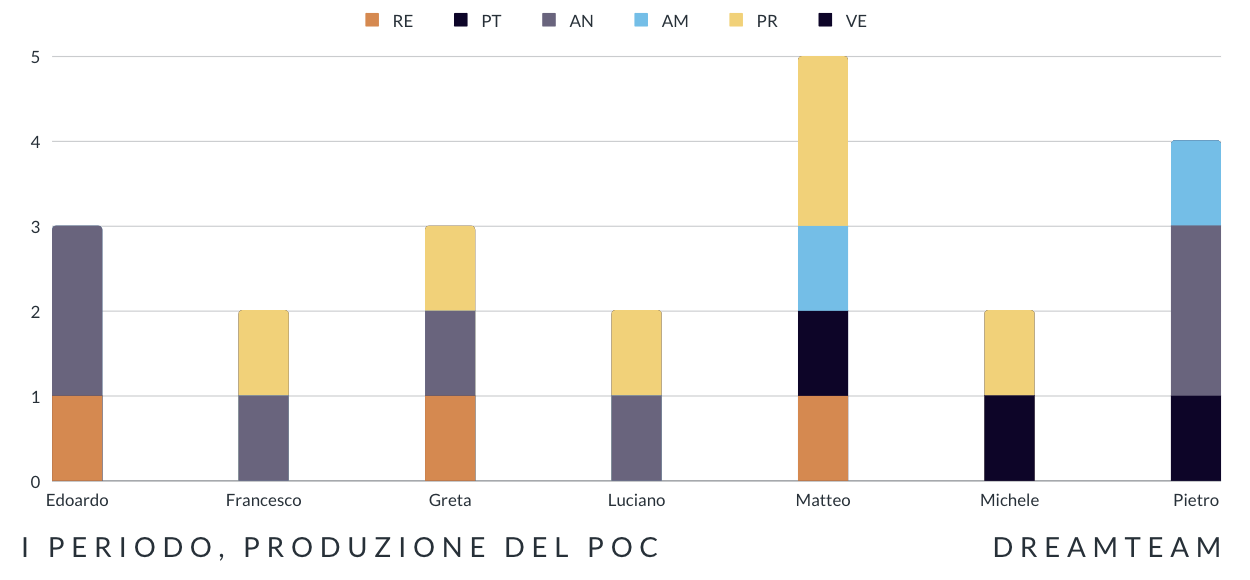
\includegraphics[scale=0.65]{Sezioni/SezioniPreventivo/grafici/Poc_I_periodo.png}
\caption{Istogramma della ripartizione delle ore durante il I periodo di produzione del PoC}
\end{figure}

\subsubsubsection{Prospetto economico}
La seguente tabella rappresenta le ore totali dedicate ad ogni ruolo e il costo in euro:

\begin{table}[H]
\begin{center}
\rowcolors{2}{gray!25}{white}
\renewcommand{\arraystretch}{1.5}
\begin{tabular}{ m{0.3\textwidth}<{\centering}  m{0.2\textwidth}<{\centering} m{0.2\textwidth}<{\centering}}
	\rowcolor{darkblue}
	\textcolor{white}{\textbf{Ruolo}}&\textcolor{white}{\textbf{Totale ore}}&\textcolor{white}{\textbf{Costo totale (\euro)}}\\ 

	Responsabile  & 3 & 90 \\	
	
	Progettista & 3 & 75 \\
	
	Analista & 7 & 175 \\

	Amministratore & 2 & 40 \\
	
	Programmatore & 6 & 90 \\
	
	Verificatore & 0 & 0 \\
	
	\textbf{Totale} & 21 & 470 \\
	
\end{tabular}
\caption{Prospetto del costo per ruoli nel I periodo della fase di produzione del PoC}
\end{center}
\end{table}

La tabella può essere rappresentata anche in forma visiva dal seguente aerogramma:
\begin{figure}[H]
\centering
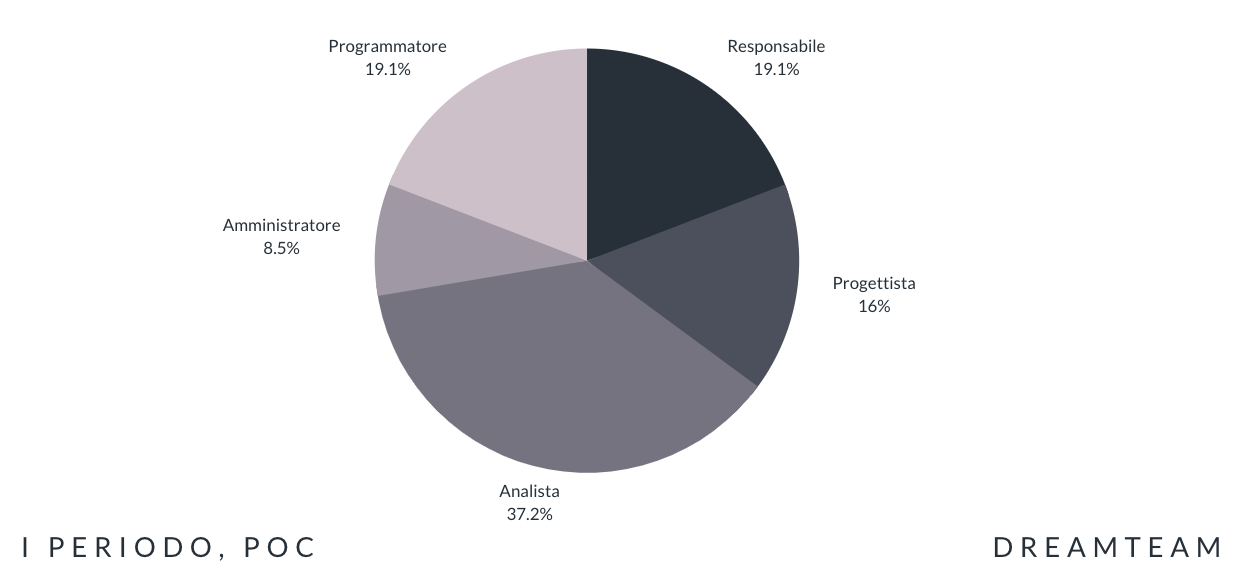
\includegraphics[scale=0.65]{Sezioni/SezioniPreventivo/grafici/Poc_I_periodo_costi.png}
\caption{Grafico a torta della ripartizione per ruolo dei costi nel I periodo della fase di produzione del PoC}
\end{figure}



\subsubsection{II Periodo}
\subsubsubsection{Prospetto orario}
La seguente tabella rappresenta la distribuzione oraria per ogni componente del gruppo nel II periodo della fase di produzione del PoC:
\begin{table}[H]
\begin{center}
\rowcolors{2}{gray!25}{white}
\renewcommand{\arraystretch}{1.25}
\begin{tabular}{ m{0.20\textwidth}<{\centering}  m{0.06\textwidth}<{\centering} m{0.06\textwidth}<{\centering} m{0.06\textwidth}<{\centering}  m{0.06\textwidth}<{\centering}  m{0.06\textwidth}<{\centering}  m{0.06\textwidth}<{\centering}  m{0.20\textwidth}<{\centering}   }
	\rowcolor{darkblue}
	\textcolor{white}{\textbf{Componente}} &\textcolor{white}{\textbf{Re}}&\textcolor{white}{\textbf{Pt}}&\textcolor{white}{\textbf{An}}&\textcolor{white}{\textbf{Am}}&\textcolor{white}{\textbf{Pr}}&\textcolor{white}{\textbf{Ve}}&\textcolor{white}{\textbf{Ore complessive}}\\ 
	Edoardo Pavan & 1 & 1 & 3 & 1 & 0 & 2 & 8 \\	
	
	Francesco Protopapa & 0 & 2 & 3 & 0 & 5 & 2 & 12 \\

	Greta Cavedon & 1 & 2 & 3 & 0 & 3 & 2 & 11 \\
	
	Luciano Wu & 0 & 2 & 3 & 0 & 4 & 3 & 12\\
	
	Matteo Basso & 1 & 3 & 0 & 0 & 4 & 2 & 10 \\
	
	Michele Gatto &  0 & 1 & 0 & 2 & 1 & 9 & 13\\
	
	Pietro Villatora & 2 & 1 & 3 & 1 & 0 & 3 & 10 \\
	
	\textbf{Ore totali ruolo} & 5 & 12 & 15 & 4 & 17 & 23 & 76\\

\end{tabular}
\caption{Distribuzione oraria per ogni componente nel II periodo della fase di produzione del PoC}
\end{center}
\end{table}

La tabella può essere rappresentata anche in forma visiva dal seguente grafico:
\begin{figure}[H]
\centering
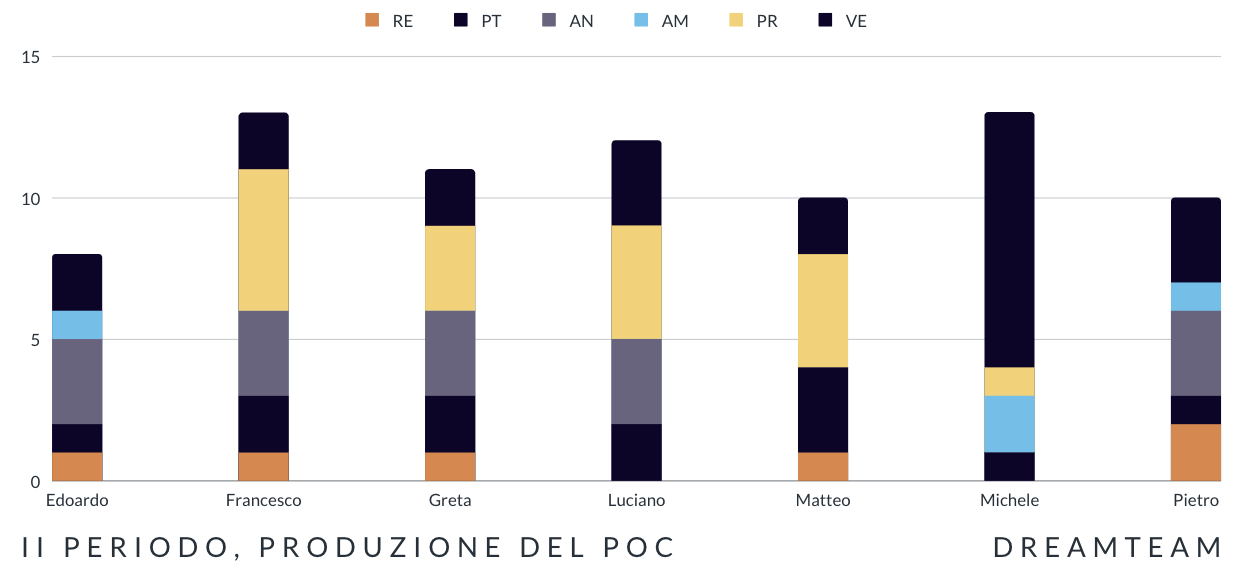
\includegraphics[scale=0.65]{Sezioni/SezioniPreventivo/grafici/Poc_II_periodo.png}
\caption{Istogramma della ripartizione delle ore durante il II periodo di produzione del PoC}
\end{figure}

\subsubsubsection{Prospetto economico}
La seguente tabella rappresenta le ore totali dedicate ad ogni ruolo e il costo in euro:

\begin{table}[H]
\begin{center}
\rowcolors{2}{gray!25}{white}
\renewcommand{\arraystretch}{1.5}
\begin{tabular}{ m{0.3\textwidth}<{\centering}  m{0.2\textwidth}<{\centering} m{0.2\textwidth}<{\centering}}
	\rowcolor{darkblue}
	\textcolor{white}{\textbf{Ruolo}}&\textcolor{white}{\textbf{Totale ore}}&\textcolor{white}{\textbf{Costo totale (\euro)}}\\ 

	Responsabile  & 5 & 150 \\	
	
	Progettista & 12 & 300 \\
	
	Analista & 15 & 375 \\

	Amministratore & 4 & 80 \\
	
	Programmatore & 17 & 255 \\
	
	Verificatore & 23 & 345 \\
	
	\textbf{Totale} & 76 & 1505 \\
	
\end{tabular}
\caption{Prospetto del costo per ruoli nel II periodo della fase di produzione del PoC}
\end{center}
\end{table}

La tabella può essere rappresentata anche in forma visiva dal seguente aerogramma:
\begin{figure}[H]
\centering
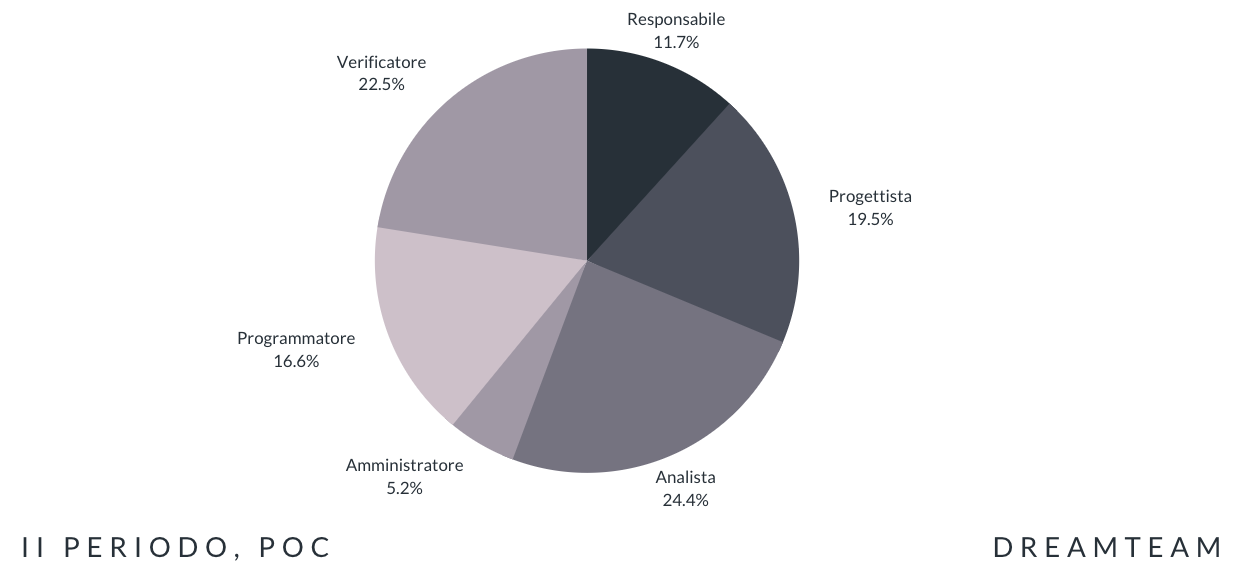
\includegraphics[scale=0.65]{Sezioni/SezioniPreventivo/grafici/Poc_II_periodo_costi.png}
\caption{Grafico a torta della ripartizione per ruolo dei costi nel II periodo della fase di produzione del PoC}
\end{figure}



\subsubsection{III Periodo}
\subsubsubsection{Prospetto orario}
La seguente tabella rappresenta la distribuzione oraria per ogni componente del gruppo nel III periodo della fase di produzione del PoC:
\begin{table}[H]
\begin{center}
\rowcolors{2}{gray!25}{white}
\renewcommand{\arraystretch}{1.25}
\begin{tabular}{ m{0.20\textwidth}<{\centering}  m{0.06\textwidth}<{\centering} m{0.06\textwidth}<{\centering} m{0.06\textwidth}<{\centering}  m{0.06\textwidth}<{\centering}  m{0.06\textwidth}<{\centering}  m{0.06\textwidth}<{\centering}  m{0.20\textwidth}<{\centering}   }
	\rowcolor{darkblue}
	\textcolor{white}{\textbf{Componente}} &\textcolor{white}{\textbf{Re}}&\textcolor{white}{\textbf{Pt}}&\textcolor{white}{\textbf{An}}&\textcolor{white}{\textbf{Am}}&\textcolor{white}{\textbf{Pr}}&\textcolor{white}{\textbf{Ve}}&\textcolor{white}{\textbf{Ore complessive}}\\ 
	Edoardo Pavan & 1 & 1 & 0 & 0 & 0 & 0 & 2 \\	
	
	Francesco Protopapa & 1 & 0 & 0 & 0 & 0 & 0 & 1 \\

	Greta Cavedon & 1 & 0 & 0 & 0 & 0 & 0 & 1 \\
	
	Luciano Wu & 0 & 1 & 0 & 0 & 0 & 0 & 1\\
	
	Matteo Basso & 1 & 0 & 0 & 0 & 0 & 0 & 1 \\
	
	Michele Gatto &  1 & 0 & 0 & 1 & 0 & 1 & 3\\
	
	Pietro Villatora & 0 & 0 & 1 & 0 & 0 & 1 & 1 \\
	
	\textbf{Ore totali ruolo} & 5 & 2 & 1 & 1 & 0 & 1 & 10\\

\end{tabular}
\caption{Distribuzione oraria per ogni componente nel III periodo della fase di produzione del PoC}
\end{center}
\end{table}

La tabella può essere rappresentata anche in forma visiva dal seguente grafico:
\begin{figure}[H]
\centering
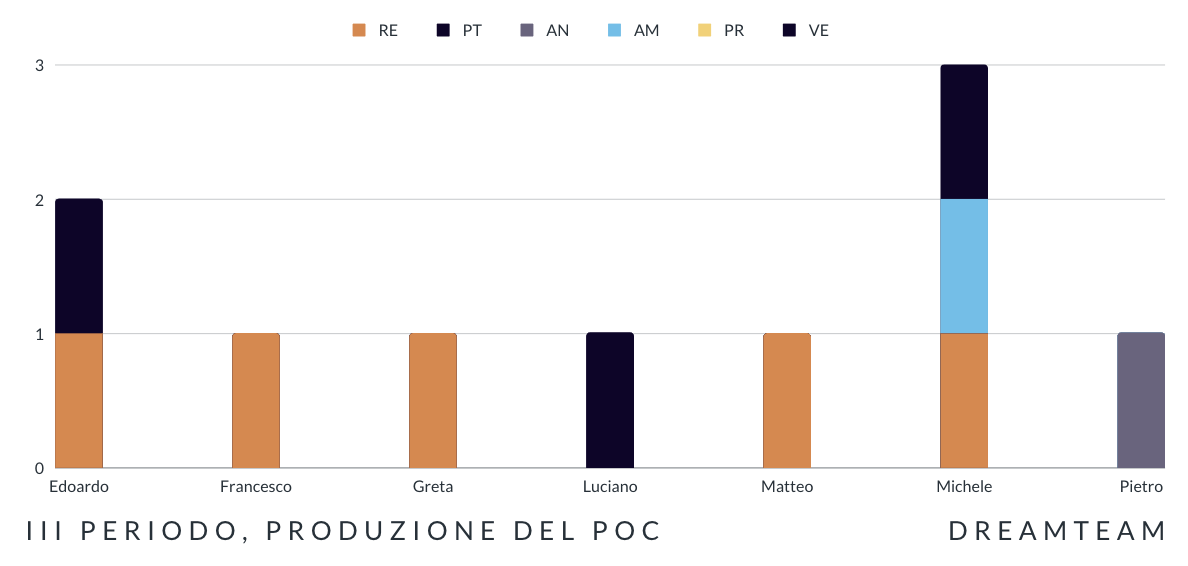
\includegraphics[scale=0.65]{Sezioni/SezioniPreventivo/grafici/Poc_III_periodo.png}
\caption{Istogramma della ripartizione delle ore durante il III periodo di produzione del PoC}
\end{figure}

\subsubsubsection{Prospetto economico}
La seguente tabella rappresenta le ore totali dedicate ad ogni ruolo e il costo in euro:

\begin{table}[H]
\begin{center}
\rowcolors{2}{gray!25}{white}
\renewcommand{\arraystretch}{1.5}
\begin{tabular}{ m{0.3\textwidth}<{\centering}  m{0.2\textwidth}<{\centering} m{0.2\textwidth}<{\centering}}
	\rowcolor{darkblue}
	\textcolor{white}{\textbf{Ruolo}}&\textcolor{white}{\textbf{Totale ore}}&\textcolor{white}{\textbf{Costo totale (\euro)}}\\ 

	Responsabile  & 5 & 150\\	
	
	Progettista & 2 & 50\\
	
	Analista & 1 & 25 \\

	Amministratore & 1 & 20 \\
	
	Programmatore & 0 & 0 \\
	
	Verificatore & 1 & 15 \\
	
	\textbf{Totale} & 10 & 260 \\
	
\end{tabular}
\caption{Prospetto del costo per ruoli nel III periodo della fase di produzione del PoC}
\end{center}
\end{table}

La tabella può essere rappresentata anche in forma visiva dal seguente aerogramma:
\begin{figure}[H]
\centering
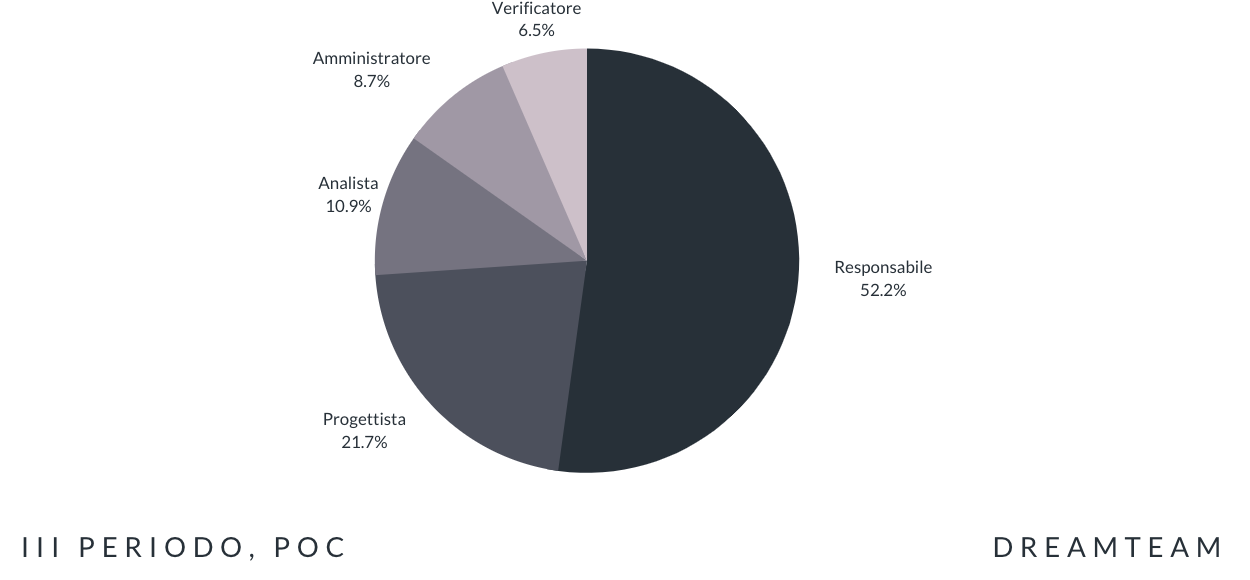
\includegraphics[scale=0.65]{Sezioni/SezioniPreventivo/grafici/Poc_III_periodo_costi.png}
\caption{Grafico a torta della ripartizione per ruolo dei costi nel III periodo della fase di produzione del PoC}
\end{figure}



\subsubsection{Fase complessiva}
\subsubsubsection{Prospetto orario}
La seguente tabella rappresenta la distribuzione oraria per ogni componente del gruppo nella fase di produzione del PoC:
\begin{table}[H]
\begin{center}
\rowcolors{2}{gray!25}{white}
\renewcommand{\arraystretch}{1.25}
\begin{tabular}{ m{0.20\textwidth}<{\centering}  m{0.06\textwidth}<{\centering} m{0.06\textwidth}<{\centering} m{0.06\textwidth}<{\centering}  m{0.06\textwidth}<{\centering}  m{0.06\textwidth}<{\centering}  m{0.06\textwidth}<{\centering}  m{0.20\textwidth}<{\centering}   }
	\rowcolor{darkblue}
	\textcolor{white}{\textbf{Componente}} &\textcolor{white}{\textbf{Re}}&\textcolor{white}{\textbf{Pt}}&\textcolor{white}{\textbf{An}}&\textcolor{white}{\textbf{Am}}&\textcolor{white}{\textbf{Pr}}&\textcolor{white}{\textbf{Ve}}&\textcolor{white}{\textbf{Ore complessive}}\\ 
	Edoardo Pavan & 4 & 2 & 5 & 1 & 0 & 2 & 14 \\	
	
	Francesco Protopapa & 1 & 2 & 4 & 0 & 6 & 2 & 15 \\

	Greta Cavedon & 3 & 2 & 4 & 0 & 4& 2 & 15 \\
	
	Luciano Wu & 0 & 3 & 4 & 0 & 5 & 3 & 15\\
	
	Matteo Basso & 2 & 4 & 0 & 1 & 6 & 2 & 15 \\
	
	Michele Gatto & 1 & 2 & 0 & 3 & 2 & 10 & 18\\
	
	Pietro Villatora & 2 & 2 & 6 & 2 & 0 & 3 & 15 \\
	
	\textbf{Ore totali ruolo} & 13 & 17 & 23 & 7 & 23 & 24 & 107\\

\end{tabular}
\caption{Distribuzione oraria per ogni componente nella fase di produzione del PoC}
\end{center}
\end{table}

La tabella può essere rappresentata anche in forma visiva dal seguente grafico:
\begin{figure}[H]
\centering
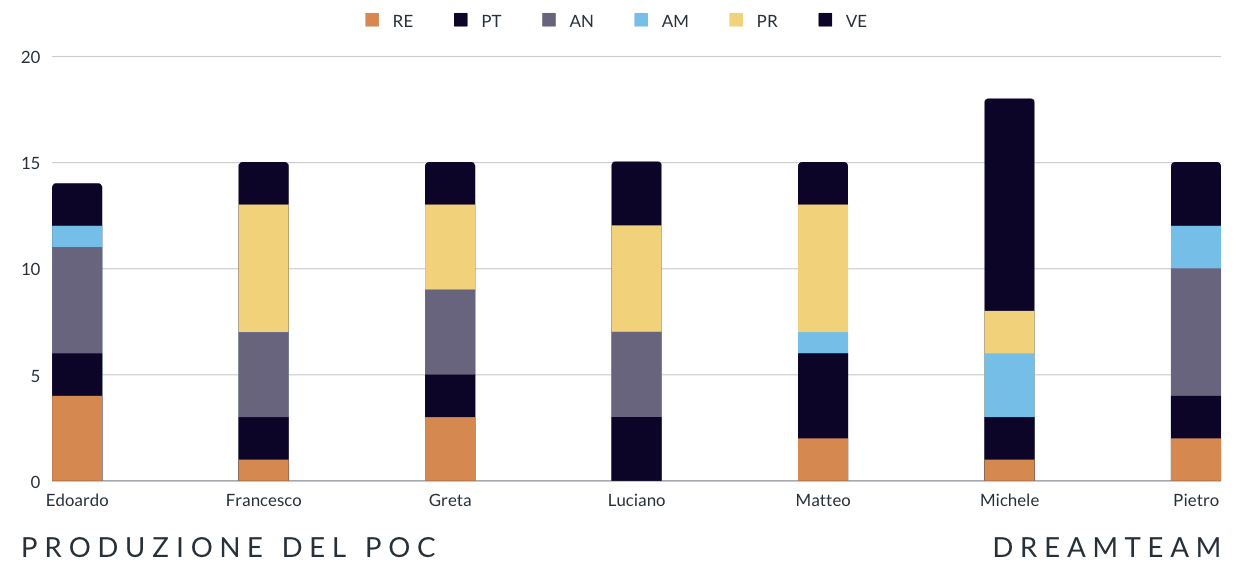
\includegraphics[scale=0.65]{Sezioni/SezioniPreventivo/grafici/Poc.png}
\caption{Istogramma della ripartizione delle ore nella fase di produzione del PoC}
\end{figure}

\subsubsubsection{Prospetto economico}
La seguente tabella rappresenta le ore totali dedicate ad ogni ruolo e il costo in euro:

\begin{table}[H]
\begin{center}
\rowcolors{2}{gray!25}{white}
\renewcommand{\arraystretch}{1.5}
\begin{tabular}{ m{0.3\textwidth}<{\centering}  m{0.2\textwidth}<{\centering} m{0.2\textwidth}<{\centering}}
	\rowcolor{darkblue}
	\textcolor{white}{\textbf{Ruolo}}&\textcolor{white}{\textbf{Totale ore}}&\textcolor{white}{\textbf{Costo totale (\euro)}}\\ 

	Responsabile  & 13 & 390\\	
	
	Progettista & 17 & 425\\
	
	Analista & 23 & 575 \\

	Amministratore & 7 & 140\\
	
	Programmatore & 23 & 345 \\
	
	Verificatore & 24 & 360 \\
	
	\textbf{Totale} & 107 & 2235 \\
	
\end{tabular}
\caption{Prospetto del costo per ruoli nella fase di produzione del PoC}
\end{center}
\end{table}

La tabella può essere rappresentata anche in forma visiva dal seguente aerogramma:

\begin{figure}[H]
\centering
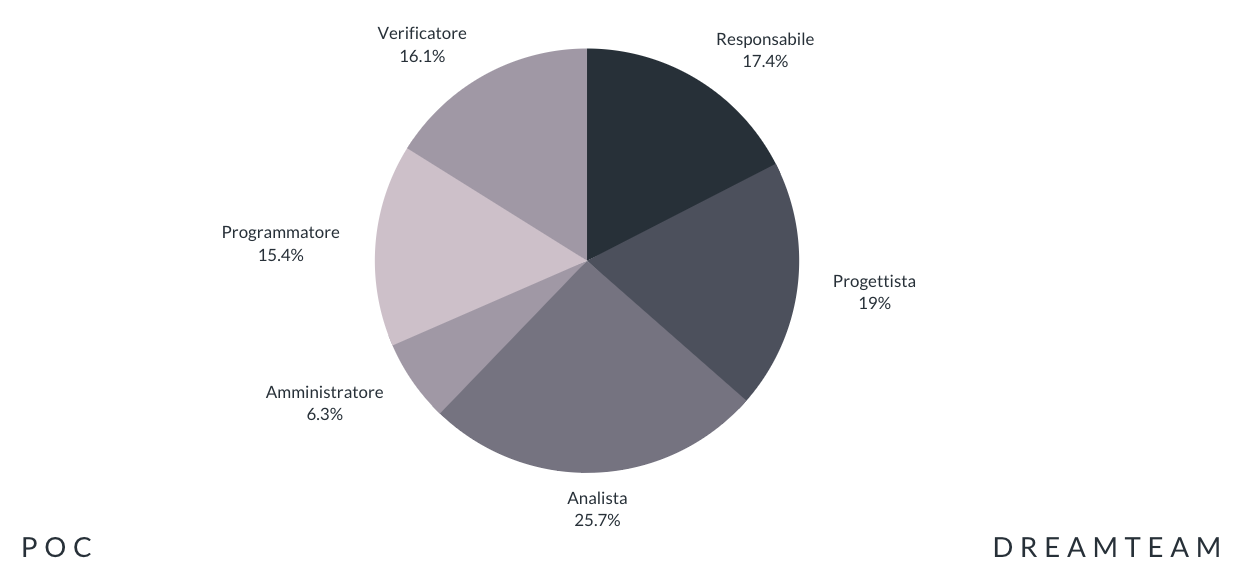
\includegraphics[scale=0.65]{Sezioni/SezioniPreventivo/grafici/Poc_costi.png}
\caption{Grafico a torta della ripartizione per ruolo dei costi nella fase di produzione del PoC}
\end{figure}